\chapter{Breast Cancer Data Analysis}

The Holy Grail of molecular biology is \cite{setubal1997introduction}

Level 3 array based data downloaded from the TCGA database
Platform for methylation data - Illumina Infinium Human DNA Methylation 450

https://portal.gdc.cancer.gov/projects/TCGA-BRCA

Hui Xiao, PhD student in the Computer Laboratory at the University of Cambridge
Antonella Iuliano, PhD student in the Department of Mathematics at the University of Salerno

\section{Epigenetic datasets used}

\section{Gene network used}

\section{Regression methods and setup}

\section{Mapping summary}

\pagebreak
%\ref{tab:map_errors}
\begin{table}[H]
	\begin{center}
		\caption{Summary of the mean squared test errors for both datasets}
		\label{tab:map_errors}
		\setlength{\tabcolsep}{18pt}
		\pgfplotstabletypeset[
		multicolumn names,
		col sep=comma,
		header=has colnames,
		display columns/0/.style={string type, column type = {l}},
		display columns/1/.style={string type, column type = {l}},
		display columns/2/.style={column type={S}, string type, column type = {r}},
		display columns/3/.style={column type={S}, column name={$\sigma_{MSE}$}, string type, column type = {r}},
		every head row/.style={
			before row={\toprule}, 
			after row/.add={}{
				\midrule\midrule
			}
		},
		every last row/.style={
			after row=\bottomrule
		},
		every nth row={5}{before row=\midrule},
		]{tables/mapping_errors.csv}
	\end{center}
\end{table}
\begin{figure}[H]
	\centering
	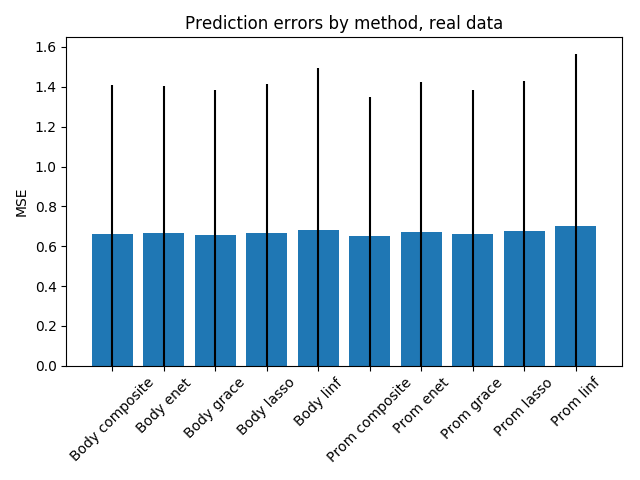
\includegraphics[scale=0.8]{mappings/errors}
	\caption{MSE by regression method and dataset}
	\label{fig:map_errors}
\end{figure}

\pagebreak
%\ref{tab:map_summary}
\begin{table}[H]
	\begin{center}
		\caption{Summary of expression-methylation mappings for both datasets and all considered regression methods; resolved refers to the number of genes with found dependencies to the methylation of others; influencing refers to the number of genes whose methylation affects the expression of others}
		\label{tab:map_summary}
		\pgfplotstabletypeset[
		multicolumn names,
		col sep=comma,
		header=has colnames,
		display columns/0/.style={string type, column type = {l}},
		display columns/1/.style={string type, column type = {l}},
		display columns/2/.style={column type={S}, string type, column type = {|r}},
		display columns/3/.style={column type={S}, string type, column type = {r}},
		display columns/4/.style={column type={S}, string type, column type = {|r}},
		display columns/5/.style={column type={S}, string type, column type = {r}},
		every head row/.style={
			before row={\toprule}, 
			after row/.add={}{
				\midrule\midrule
			}
		},
		every last row/.style={
			after row=\bottomrule
		},
		every nth row={5}{before row=\midrule},
		]{tables/mapping_summary.csv}
	\end{center}
\end{table}
\begin{figure}[H]
	\centering
	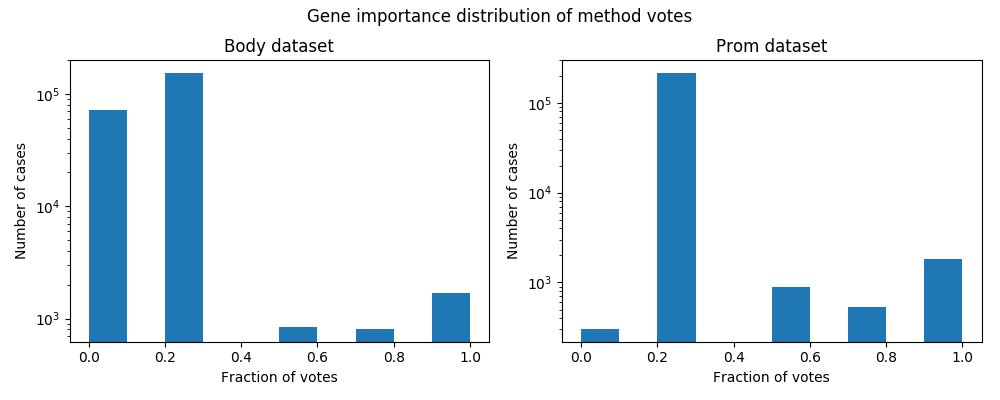
\includegraphics[scale=0.54]{mappings/vote_distribution}
	\caption{Predictor importance fraction of votes distribution for cell body (left) and promoter (right) datasets}
	\label{fig:map_vote_dist}
\end{figure}


\pagebreak
\subsection{Lasso}

\begin{figure}[H]
	\centering
	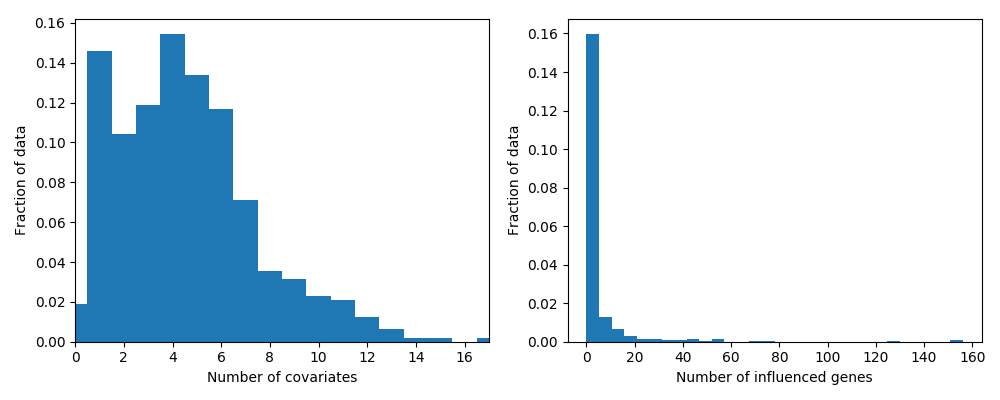
\includegraphics[scale=0.54]{mappings/distributions/Lasso_Body}
	\caption{Lasso mapping dependencies summary for cell body dataset}
	\label{fig:map_body_lasso}
\end{figure}

\begin{figure}[H]
	\centering
	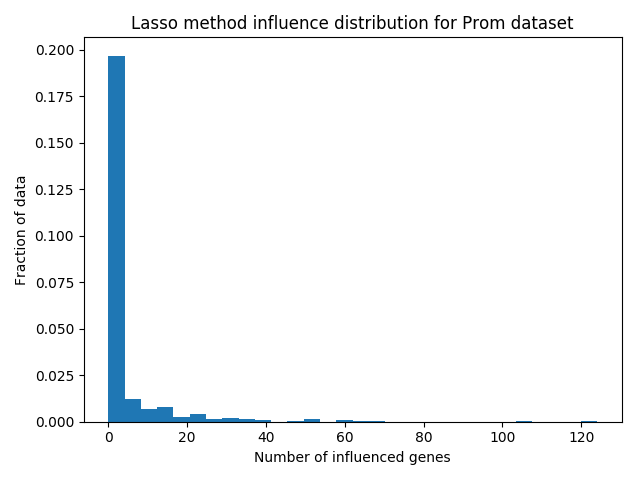
\includegraphics[scale=0.54]{mappings/distributions/Lasso_Prom}
	\caption{Lasso mapping dependencies summary for promoter dataset}
	\label{fig:map_prom_lasso}
\end{figure}


\pagebreak
\subsection{Elastic Net}

\begin{figure}[H]
	\centering
	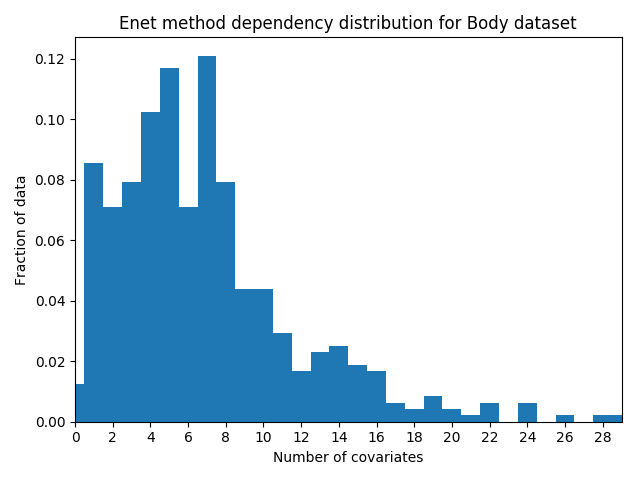
\includegraphics[scale=0.54]{mappings/distributions/Enet_Body}
	\caption{Elastic Net mapping dependencies summary for cell body dataset}
	\label{fig:map_body_enet}
\end{figure}

\begin{figure}[H]
	\centering
	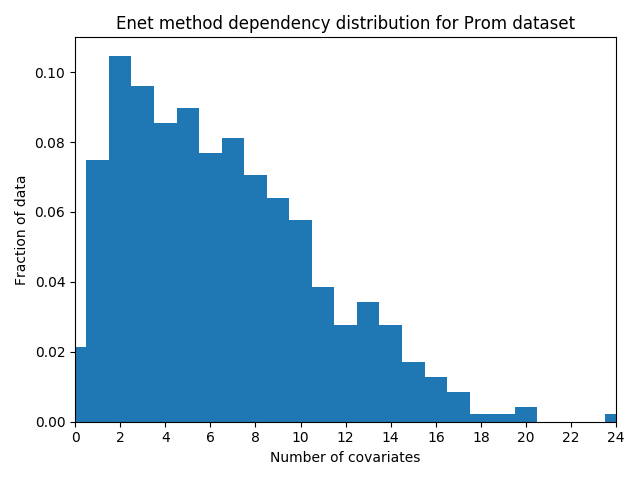
\includegraphics[scale=0.54]{mappings/distributions/Enet_Prom}
	\caption{Elastic Net mapping dependencies summary for promoter dataset}
	\label{fig:map_prom_enet}
\end{figure}


\pagebreak
\subsection{Grace}

\begin{figure}[H]
	\centering
	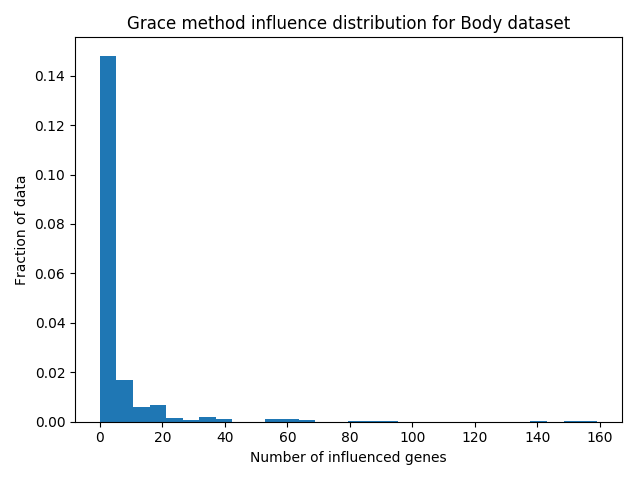
\includegraphics[scale=0.54]{mappings/distributions/Grace_Body}
	\caption{Grace mapping dependencies summary for cell body dataset}
	\label{fig:map_body_grace}
\end{figure}

\begin{figure}[H]
	\centering
	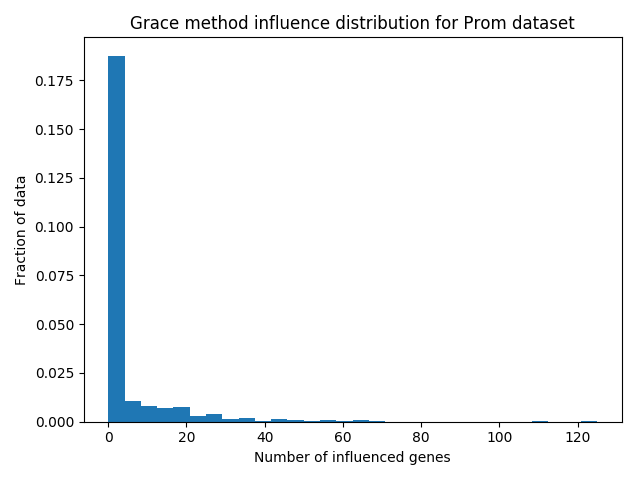
\includegraphics[scale=0.54]{mappings/distributions/Grace_Prom}
	\caption{Grace mapping dependencies summary for promoter dataset}
	\label{fig:map_prom_grace}
\end{figure}


\pagebreak
\subsection{Linf}

\begin{figure}[H]
	\centering
	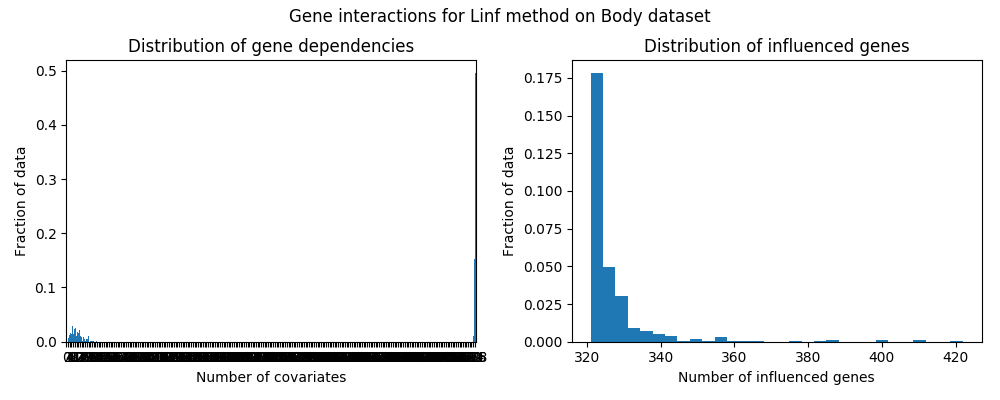
\includegraphics[scale=0.54]{mappings/distributions/Linf_Body}
	\caption{Linf mapping dependencies summary for cell body dataset}
	\label{fig:map_body_linf}
\end{figure}

\begin{figure}[H]
	\centering
	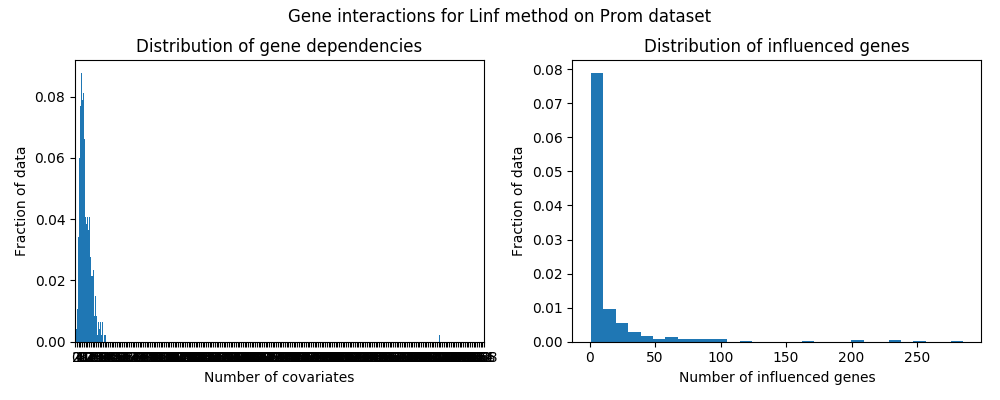
\includegraphics[scale=0.54]{mappings/distributions/Linf_Prom}
	\caption{Linf mapping dependencies summary for promoter dataset}
	\label{fig:map_prom_linf}
\end{figure}


\pagebreak
\subsection{Composite}

\begin{figure}[H]
	\centering
	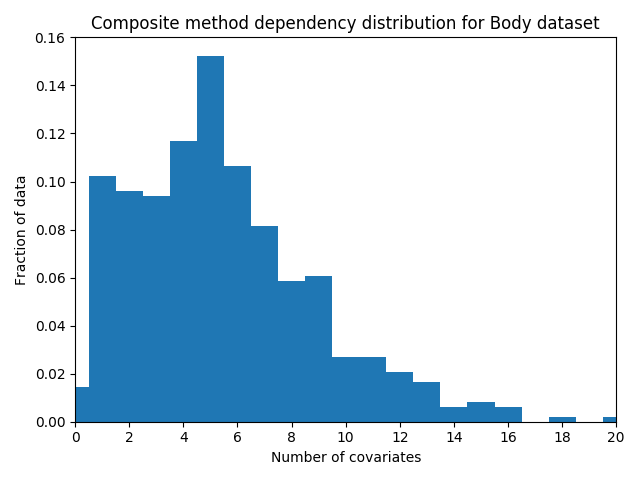
\includegraphics[scale=0.54]{mappings/distributions/Composite_Body}
	\caption{Composite method mapping dependencies summary for cell body dataset}
	\label{fig:map_body_comp}
\end{figure}

\begin{figure}[H]
	\centering
	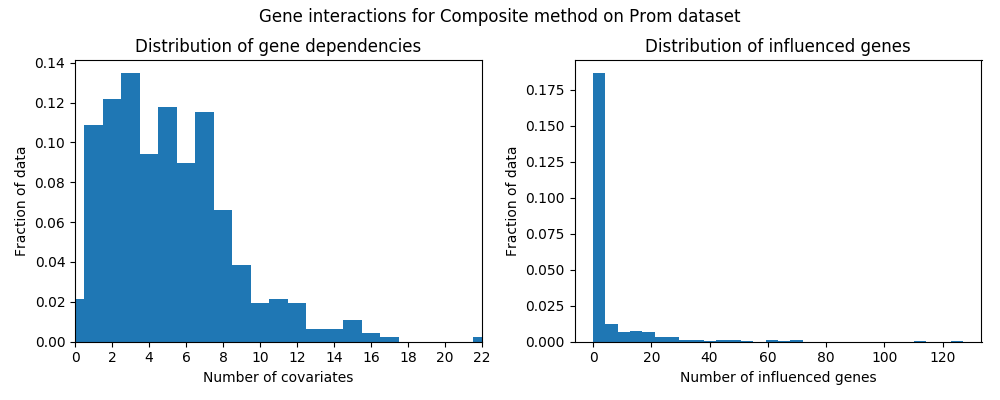
\includegraphics[scale=0.54]{mappings/distributions/Composite_Prom}
	\caption{Composite method mapping dependencies summary for promoter dataset}
	\label{fig:map_prom_comp}
\end{figure}